%!TeX root=../main.tex

\chapter{Conceitos Fundamentais}
\label{cap:conceitos}

\section[Shogi]{Shogi}
    O shogi é um jogo de tabuleiro disputado em um tabuleiro com 9 linhas e 9 colunas. O jogo utiliza 8 tipos de peças, das quais 6 podem assumir formas promovidas (que possuem movimentações diferentes das versões padrão), totalizando 14 tipos de peças. A notação ocidental das peças e seus respectivos símbolos japoneses são apresentados na Tabela~\ref{tab:shogi_pieces}.

    A notação ocidental utilizada em publicações de língua inglesa foi desenvolvida por \cite{hodges-notation}, com base em elementos da notação algébrica do xadrez. 
\section{Convenções de shogi}
\begin{table}[H]
	\centering
	\caption{Correspondência entre as notações japonesa e ocidental das peças de shogi}
	\label{tab:shogi_pieces}
	\begin{tabular}{c c c}
		\toprule
		\textbf{Símbolo} & \textbf{Notação ocidental} & \textbf{Peça} \\
		\midrule
		歩 & P & Peão \\
		香 & L  & Lança \\
		桂 & N  & Cavalo \\
		銀 & S  & General de Prata \\
		金 & G  & General de Ouro \\
		角 & B  & Bispo \\
		飛 & R  & Torre \\
		玉 & K  & Rei \\
		と & +P  & Peão Promovido \\
		成香 & +L  & Lança Promovida \\
		成桂 & +N  & Cavalo Promovido \\
		成銀 & +S  & General de Prata Promovido \\
		馬 & +B  & Bispo Promovido \\
		龍 ou 竜 & +R  & Torre Promovida \\
		\bottomrule
	\end{tabular}
\end{table}
\begin{itemize}
	\item \textbf{Jogadores}: os jogadores são definidos como preto (\textit{sente}), quem faz o primeiro movimento, ou branco (\textit{gote}).
	\item \textbf{Casas}: as colunas são numeradas de 1 a 9, da direita para a esquerda, e as linhas são identificadas com letras de a a i, de cima para baixo, considerando o ponto de vista do sente.
	\item \textbf{Posição}: uma casa é identificada pela combinação do número da coluna com a letra da linha. Por exemplo, 5a corresponde à casa localizada na coluna 5 e na primeira linha.
	\begin{table}[H]
		\centering
		\caption{Movimentos das peças}
		\label{tab:pieces_movements}
		\begin{tabular}{c p{9cm}}
			\toprule
			\textbf{Peça} & \textbf{Movimento}\\
			\midrule
			Peão & Uma casa para a frente. \\
			Lança & Qualquer número de casas para a frente. \\
			Cavalo & Salta para uma das duas casas duas fileiras à frente e uma coluna para um dos lados. \\
			General de prata & Uma casa na diagonal ou uma casa para a frente. \\
			General de ouro & Uma casa para a frente, para trás ou para os lados, ou uma casa na diagonal para a frente. \\
			Bispo & Qualquer número de casas na diagonal. \\
			Torre & Qualquer número de casas na horizontal ou vertical. \\
			Rei & Uma casa em qualquer direção. \\
			Peão promovido & Como um general de ouro. \\
			Lança promovida & Como um general de ouro. \\
			Cavalo promovido & Como um general de ouro. \\
			General de prata promovido & Como um general de ouro. \\
			Bispo promovido & Como um bispo ou uma casa na horizontal ou vertical. \\
			Torre promovida & Como uma torre ou uma casa na diagonal. \\
			\bottomrule
		\end{tabular}
	\end{table}
	\item \textbf{Movimentos}\textsuperscript{\cite{shogi-rules}}: o sistema adota uma variação da convenção de Hodges, com adaptações para facilitar a compreensão por iniciantes. Os movimentos de cada peça se encontram na Tabela~\ref{tab:pieces_movements}. Um movimento é considerado legal quando segue as regras do jogo descritas abaixo.
		\begin{itemize}
			\item \textbf{Deslocamento}: [Origem]->[Destino]. Por exemplo, \textbf{9g->9f} se refere ao movimento da casa \textbf{9g} para a casa \textbf{9f}. Na notação de referência, o deslocamento não possui o símbolo "->".
			\item \textbf{Captura}: quando aplicável, o movimento ocupa a casa da peça adversária capturada, que é removida do tabuleiro e passa a pertenceraà mão jogador que realizou a captura.
			\item \textit{\textbf{Drop}}: [Peça]*[Posição]. Refere-se à recolocação no tabuleiro de uma peça capturada anteriormente. Por exemplo, \textbf{P*9e} representa a colocação de um peão na casa \textbf{9e}.
			\item \textbf{Promoção}: [Origem]->[Destino]+. O símbolo "+" representa que a peça foi promovida ao final do movimento. Por exemplo, \textbf{9d->9c+} representa o movimento da casa \textbf{9d} para a casa \textbf{9c}, seguido de sua promoção. A promoção pode ocorrer quando a origem ou destino do movimento está dentro da zona de promoção, que corresponde às três fileiras mais distantes do jogador. Em determinadas situações ela é obrigatória: por exemplo, um peão ou uma lança que alcança a última fileira, ou um cavalo que alcança uma das duas últimas fileiras, pois não possuem movimentos legais a partir dessas posições. 
		\end{itemize}
	\item \textbf{Xeque}: Um Rei está em \textbf{xeque} quando pode ser capturado por uma ou mais peças do oponente. O jogador ameaçado deve realizar um movimento legal que elimine essa ameaça.
	\item \textbf{Xeque-mate}: Um Rei está em \textbf{xeque-mate} quando ele está em xeque e não existe um movimento legal que elimine o xeque. Nessa situação, a vitória pertence ao jogador que causou o xeque-mate.
\end{itemize}

\section{Representação SFEN}
No shogi, a \textit{Shogi Forsyth–Edwards Notation} (SFEN)\textsuperscript{\cite{USI}} é utilizada para representar textualmente uma posição no jogo. Essa representação é composta por quatro campos separados por espaços:
\begin{itemize}
	\item Tabuleiro: disposição das peças nas casas;
	\item Turno: jogador que deve realizar o próximo movimento, b para o \textit{sente} e w para o \textit{gote};
	\item Peças nas mãos: peças capturadas que podem ser reutilizadas por quem fez a captura;
	\item Número do movimento: contador do movimento atual.
\end{itemize}

\begin{figure}[H]
	\centering
	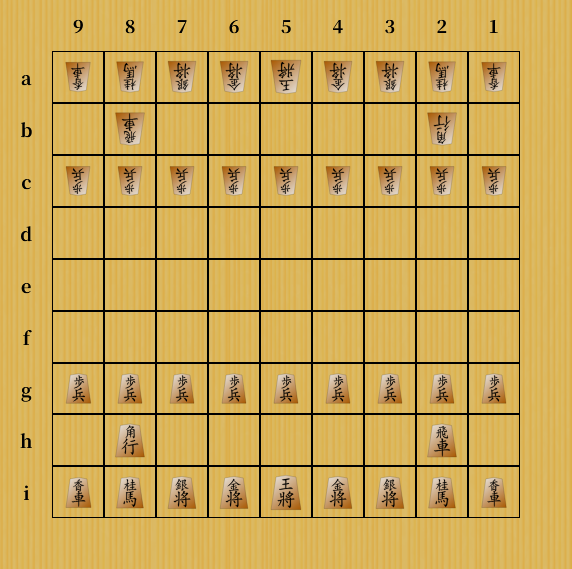
\includegraphics[width=0.9\linewidth]{images/board.png}
	\caption{Posição inicial do tabuleiro}
	\label{fig:posicao_inicial}
\end{figure}

Considere a seguinte representação SFEN correspondente à posição inicial do tabuleiro: 

\begin{center}
\small
\texttt{lnsgkgsnl/1r5b1/ppppppppp/9/9/9/PPPPPPPPP/1B5R1/LNSGKGSNL b - 1}
\end{center}
Como ilustrado na Figura~\ref{fig:posicao_inicial}, o primeiro campo descreve o tabuleiro, 
cujas linhas são separadas pelo caractere "/" e estão ordenadas de cima para baixo. As peças 
seguem a notação da Tabela~\ref{tab:shogi_pieces}. As letras minúsculas representam as peças 
do \textit{gote} e as maiúsculas representam as peças do \textit{sente}. Casas vazias são 
representadas por números que indicam a quantidade de casas consecutivas desocupadas.

O segundo campo indica que o \textit{sente} deve fazer o próximo movimento, uma vez que 
ele é o jogador que começa o jogo. O símbolo - no terceiro campo indica que nenhum deles 
possui peças capturadas disponíveis para reutilização. Por fim, o quarto campo indica que 
a próxima jogada será a primeira do jogo.
	
\section{Universal Shogi Interface}
\label{sec:USI}
No contexto do shogi computacional, os chamados motores, ou \textit{engines}, são programas 
capazes de analisar posições e buscar movimentos possíveis, utilizando algoritmos de busca 
e funções de avaliação para estimar a qualidade de diferentes jogadas. Esses motores podem 
ser integrados a interfaces gráficas, permitindo o desenvolvimento de aplicações de análise 
de partidas, como o Lishogi, que utiliza o YaneuraOu\textsuperscript{\cite{yaneuraou}}.

A comunicação entre motores e interfaces pode ser realizada por meio do protocolo 
\textit{Universal Shogi Interface} (USI), baseado no protocolo equivalente utilizado 
no xadrez \textit{Universal Chess Interface} (UCI). Ao padronizar comandos e respostas, 
o USI elimina a necessidade de implementar os mecanismos de análise dentro das próprias aplicações.

Esse protocolo define operações para inicializar o motor, configurar suas opções, fornecer 
posições do tabuleiro por meio da representação SFEN e solicitar a busca por movimentos. 
Essa comunicação ocorre através da entrada e da saída padrão do processo do motor. Durante 
uma busca, o programa pode retornar informações sobre a análise realizada, como a profundidade 
alcançada que indica quantos meios-lances (movimentos individuais de um jogador) foram explorados 
na busca, a avaliação da posição e os movimentos candidatos considerados. 